\documentclass[11pt,a4paper]{article}

% Fonts and encoding
\usepackage{fontspec}
\usepackage{polyglossia}
\setmainlanguage{english}

% Page geometry
\usepackage[margin=2.5cm]{geometry}

% Math
\usepackage{amsmath}
\usepackage{amssymb}

% Graphics
\usepackage{graphicx}
\usepackage{float}
\graphicspath{{../figures/}}

% Tables
\usepackage{booktabs}
\usepackage{tabularx}
\usepackage{multirow}

% Hyperlinks
\usepackage{hyperref}
\hypersetup{
    colorlinks=true,
    linkcolor=blue,
    citecolor=blue,
    urlcolor=blue
}

% Bibliography
\usepackage[backend=bibtex,style=authoryear,sorting=nyt,maxnames=3]{biblatex}
\addbibresource{references.bib}

% Line spacing
\usepackage{setspace}
\onehalfspacing

% Section formatting
\usepackage{titlesec}
\titleformat{\section}{\large\bfseries}{\thesection.}{0.5em}{}
\titleformat{\subsection}{\normalsize\bfseries}{\thesubsection.}{0.5em}{}

% Headers
\usepackage{fancyhdr}
\pagestyle{fancy}
\fancyhf{}
\fancyhead[L]{\small Empirical Estimation of CES Elasticity of Substitution}
\fancyhead[R]{\small\thepage}

\begin{document}

\begin{center}
{\LARGE\bfseries Empirical Estimation of CES Elasticity of Substitution\\
for AI-Augmented Production: OECD Panel Evidence\\
and Agent-Based Model Sensitivity}

\vspace{0.8cm}

{\large Mateusz Maciaszek}

\vspace{0.3cm}

{\small February 2026}

\vspace{0.5cm}

\begin{minipage}{0.85\textwidth}
\small\textbf{Abstract.}
\autocite{maciaszek2026acceleration,maciaszek2026monetary} demonstrate that the interaction between universal basic income (UBI) and AI-driven automation produces phase transitions in a stock-flow consistent agent-based model (SFC-ABM) of the Polish economy.
Both papers rely on \emph{calibrated} sector-specific CES elasticities of substitution ($\sigma$) that are 5--10$\times$ larger than values found in the empirical literature.
This paper provides the missing empirical grounding.
Using an OECD panel of 30 countries $\times$ 6 sectors over 2000--2023, we estimate $\sigma$ via two independent methods: (i)~a normalized CES supply system with Arellano-Bond dynamic panel GMM \autocite{leonledesma2010identifying}, and (ii)~a hierarchical Bayesian model with informative priors from the \autocite{knoblach2020what} meta-analysis.
Robot density from the International Federation of Robotics (IFR) and ICT capital expenditure from Eurostat serve as proxies for AI-specific capital.
We show that non-market sectors (Healthcare, Public) cannot be identified via the wage equation due to the SNA cost convention ($Y \approx wL + \delta K$), which renders $\ln w \sim \ln(Y/L)$ a near-tautology; for these sectors we report literature priors from \autocite{knoblach2020what}.
For the four market sectors, both methods yield $\sigma$ estimates in the range 1.4--9.0, substantially below the calibrated values (3.0--50.0) but consistent with the meta-analytic literature.
We then re-run the ABM with empirical $\sigma$ at UBI$=2{,}000$~PLN under the PLN monetary regime.
The qualitative dynamics---adoption driven by sector-specific substitutability, dampened by NBP monetary tightening---are preserved, though adoption levels shift: from 12.95\% (calibrated) to 11.42\% (empirical) and 7.25\% (CI lower bound).
These results confirm that the acceleration paradox mechanism is robust to realistic parameterization, while highlighting that $\sigma$ calibration materially affects the quantitative predictions.

\vspace{0.3cm}
\noindent\textbf{Keywords:} CES production function, elasticity of substitution, GMM estimation, Bayesian inference, robot density, automation, agent-based model, complexity economics

\vspace{0.3cm}
\noindent\textbf{JEL:} C11, C23, E17, J23, O33
\end{minipage}
\end{center}

\vspace{0.5cm}


%% ==================================================================
\section{Introduction}
\label{sec:intro}

The CES (Constant Elasticity of Substitution) production function, introduced by \autocite{arrow1961capital}, parameterizes the ease with which capital can substitute for labor through a single parameter~$\sigma$.
When $\sigma > 1$, capital and labor are gross substitutes; automation technology reduces labor demand for a given output level.
When $\sigma < 1$, they are gross complements, and automation raises labor's marginal product.
The boundary case $\sigma = 1$ is the Cobb-Douglas function.

In \autocite{maciaszek2026acceleration}, we built an SFC-ABM of the Polish economy with 10,000 firms across 6 sectors, each characterized by a sector-specific $\sigma$ ranging from 1.0 (Public) to 50.0 (BPO/SSC).
The model produces a phase transition: below a critical UBI level, adoption remains low; above it, a feedback loop between UBI-funded consumption, firm revenue, and technology adoption drives the economy to a high-automation equilibrium.
\autocite{maciaszek2026monetary} extended the model to compare PLN and EUR monetary regimes.

A key limitation of both papers is that the $\sigma$ values were \emph{calibrated} to produce qualitatively reasonable dynamics rather than estimated from data.
The calibrated values---especially BPO/SSC at $\sigma=50$ and Manufacturing at $\sigma=10$---are far higher than the empirical consensus.
The meta-analysis by \autocite{knoblach2020what} reports aggregate $\sigma$ estimates centered around 0.5--0.8, with sector-level values rarely exceeding 3--4 even in manufacturing.

This paper addresses the gap by:
\begin{enumerate}
    \item Building an OECD panel (30 countries, 6 ABM-consistent sectors, 2000--2023) with IFR robot density and Eurostat ICT CAPEX as automation capital proxies;
    \item Estimating sector-specific $\sigma$ via normalized CES + Arellano-Bond GMM;
    \item Cross-validating with hierarchical Bayesian estimation using priors from \autocite{knoblach2020what};
    \item Re-running the ABM with empirical $\sigma$ to test robustness of the phase transition.
\end{enumerate}

The rest of the paper proceeds as follows.
Section~\ref{sec:literature} reviews the literature on CES estimation.
Section~\ref{sec:data} describes the data and sector mapping.
Section~\ref{sec:methodology} presents both estimation methods.
Section~\ref{sec:results} reports the estimates.
Section~\ref{sec:sensitivity} tests ABM sensitivity.
Section~\ref{sec:discussion} interprets the findings.
Section~\ref{sec:conclusion} concludes.


%% ==================================================================
\section{Literature Review}
\label{sec:literature}

\subsection{CES Estimation: Aggregate and Sectoral}

The CES production function has been estimated at the aggregate level since \autocite{arrow1961capital}.
Early estimates suffered from identification problems: with only two factors and Hicks-neutral technical change, $\sigma$ is not separately identified from the bias of technical progress \autocite{leonledesma2010identifying}.

\autocite{klump2007normalization} and \autocite{klump2012normalization} proposed the \emph{normalized CES} approach, which resolves the identification issue by expressing the production function relative to a base-period equilibrium.
\autocite{leonledesma2010identifying} extended this to a supply-side system of first-order conditions, allowing joint estimation of $\sigma$ and the direction of technical change via GMM.
Their aggregate US estimate is $\sigma \approx 0.6$.

At the sector level, identification is aided by cross-country variation.
\autocite{knoblach2020what} meta-analyze 3,186 estimates from 121 studies and find a mean gross $\sigma$ of 0.58 (95\% CI: 0.49--0.67) after correcting for publication bias.
The meta-regression shows that sector, estimation method, and data frequency are key moderators.
Manufacturing tends to have higher $\sigma$ than services, consistent with greater scope for physical automation.

\subsection{Robot Density as Automation Proxy}

\autocite{graetz2018robots} use IFR robot density to estimate the effect of industrial robots on productivity and wages across 17 countries (1993--2007), finding that robots raise productivity and wages but reduce labor share.
\autocite{acemoglu2020robots} apply a similar approach to US commuting zones.

The IFR data cover manufacturing in detail but have limited service-sector coverage.
We complement robot density with Eurostat ICT CAPEX, which captures software and digital automation in services, to build a composite ``automation capital'' variable that maps to all 6 ABM sectors.

\subsection{Bayesian Approaches}

Bayesian CES estimation allows incorporation of prior information from the meta-analytic literature and produces full posterior distributions that naturally quantify parameter uncertainty.
\autocite{gelman2006prior} discusses prior specification for hierarchical variance parameters.
We follow this approach with informative LogNormal priors calibrated to \autocite{knoblach2020what} sector-level means and standard deviations.


%% ==================================================================
\section{Data}
\label{sec:data}

\subsection{Sources}

We combine four data sources:

\begin{enumerate}
    \item \textbf{OECD STAN} (ISIC Rev.4): Value added, employment, gross fixed capital formation, and labor compensation by industry for 34 OECD countries, 2000--2023 \autocite{oecd2024stan}.
    \item \textbf{IFR robot density}: Robot stock per 10,000 employees by industry, available via the OECD ROBOT\_INDUSTRY dataset \autocite{ifr2024world}.
    \item \textbf{Eurostat ICT}: ICT capital expenditure by NACE sector (\texttt{isoc\_ci\_it\_en2}), covering EU countries.
    \item \textbf{GUS BDL}: Fixed assets, employment, and wages by PKD section for Poland, used as a country-specific comparison.
\end{enumerate}

\subsection{Sector Mapping}

We aggregate ISIC Rev.4 sections into the 6 ABM sectors used in \autocite{maciaszek2026acceleration}:

\begin{table}[H]
\centering
\caption{ISIC Rev.4 to ABM sector crosswalk}
\label{tab:crosswalk}
\begin{tabular}{ll}
\toprule
\textbf{ABM Sector} & \textbf{ISIC Sections} \\
\midrule
BPO/SSC & J (Information \& Communication), N (Administrative) \\
Manufacturing & C \\
Retail/Services & G, H, I, K, L, M, R, S \\
Healthcare & Q (Human Health \& Social Work) \\
Public & O (Public Administration), P (Education) \\
Agriculture & A \\
\bottomrule
\end{tabular}
\end{table}

Sections B (Mining), D (Utilities), E (Water), and F (Construction) are excluded as they do not map cleanly to the ABM's sectoral structure.

\subsection{Panel Construction}

The final OECD panel has dimensions country $\times$ sector $\times$ year.
All monetary values are deflated to constant 2015 prices using the OECD GDP deflator.
We construct:
\begin{itemize}
    \item $Y_{ist}$: real value added (sector $s$, country $i$, year $t$)
    \item $L_{ist}$: total employment
    \item $w_{ist} = \text{LABR}_{ist} / L_{ist}$: real wage per employee
    \item $K_{ist}^{\text{robot}}$: robot stock per 10,000 employees (IFR)
    \item $K_{ist}^{\text{ict}}$: ICT CAPEX (Eurostat)
    \item $K_{ist}^{\text{auto}} = K^{\text{robot}} + K^{\text{ict}}$: composite automation capital
\end{itemize}


%% ==================================================================
\section{Methodology}
\label{sec:methodology}

\subsection{Normalized CES Supply System (GMM)}

Following \autocite{leonledesma2010identifying} and \autocite{klump2012normalization}, we estimate a wage equation derived from the first-order condition of a CES production function.
For sector $s$, country $i$, year $t$:

\begin{equation}
\ln w_{ist} = \alpha_i + \beta_s \ln\left(\frac{Y_{ist}}{L_{ist}}\right) + \gamma_s \, t + u_{ist}
\label{eq:wage}
\end{equation}

where $\alpha_i$ is a country fixed effect and $\gamma_s$ captures sector-specific time trends (proxy for technical change).
The CES elasticity is recovered as:

\begin{equation}
\sigma_s = \frac{1}{1 - \beta_s}
\label{eq:sigma}
\end{equation}

\textbf{Identification.}
OLS estimation of (\ref{eq:wage}) is inconsistent because $Y/L$ (labor productivity) is endogenous---it depends on both technology shocks and labor market conditions that also affect wages.
We address this using first-differencing to eliminate $\alpha_i$ and instrumenting with twice-lagged variables:

\begin{equation}
\Delta \ln w_{ist} = \beta_s \, \Delta \ln(Y/L)_{ist} + \gamma_s + \Delta u_{ist}
\end{equation}

Instruments: $\ln(K/L)_{is,t-2}$ and $\ln(Y/L)_{is,t-2}$, following the Arellano-Bond approach \autocite{arellano1991tests}.

\textbf{Diagnostics:}
\begin{itemize}
    \item \textbf{Hansen $J$ test}: overidentification (null: instruments are valid). We require $p > 0.05$.
    \item \textbf{AR(2) test}: no second-order serial correlation in the first-differenced residuals. We require $p > 0.05$.
\end{itemize}

Standard errors for $\hat{\sigma}_s$ are obtained via the delta method:
\begin{equation}
\text{SE}(\hat{\sigma}_s) = \frac{1}{(1 - \hat{\beta}_s)^2} \cdot \text{SE}(\hat{\beta}_s)
\end{equation}

\subsection{Non-Market Sector Identification Problem}
\label{sec:sna}

The wage equation~(\ref{eq:wage}) relies on independent variation between wages~$w$ and labor productivity~$Y/L$.
In non-market sectors---Healthcare (ISIC~Q) and Public Administration/Education (ISIC~O, P)---the System of National Accounts (SNA) measures output by the cost convention: value added is defined as $Y \approx wL + \delta K$, where~$\delta K$ is the consumption of fixed capital \autocite{oecd2024sna}.
This implies $Y/L \approx w + \delta K/L$, so regressing $\ln w$ on $\ln(Y/L)$ is a near-tautology: $\beta \to 1$ and $\sigma = 1/(1-\beta) \to \infty$ mechanically, regardless of the true substitutability between labor and capital.

The OECD explicitly excludes non-market sectors from productivity analyses for this reason \autocite{oecd2024sna}.
In our OECD panel, unconstrained GMM estimation yields $\hat{\sigma} = 17.2$ for Healthcare and $\hat{\sigma} = 81.2$ for Public---values consistent with the tautology artifact, not with economic fundamentals.

For these two sectors, we therefore \emph{do not estimate} $\sigma$ from data.
Instead, we report the literature priors from \autocite{knoblach2020what} (Healthcare: $\mu=1.0$, $\tau=0.5$; Public: $\mu=0.8$, $\tau=0.4$), which are based on studies that use physical output measures or indirect identification strategies.
This market/non-market split yields a consistent 6-sector $\sigma$ vector for the ABM sensitivity analysis.

\subsection{Hierarchical Bayesian Estimation}

As a robustness check, we estimate $\sigma_s$ using a hierarchical Bayesian model that incorporates prior information from the \autocite{knoblach2020what} meta-analysis:

\begin{align}
\sigma_s &\sim \text{LogNormal}\big(\ln(\mu_s^{\text{prior}}), \, \tau_s^{\text{prior}}\big) \label{eq:prior} \\
\beta_s &= 1 - 1/\sigma_s \\
\ln w_{ist} &\sim \mathcal{N}\big(\alpha_i + \beta_s \ln(Y/L)_{ist} + \gamma_s \, t, \; \sigma_\varepsilon\big) \\
\alpha_i &\sim \mathcal{N}(0, \sigma_\alpha) \label{eq:hierarchical}
\end{align}

The priors in (\ref{eq:prior}) are sector-specific, with means and standard deviations drawn from Table~\ref{tab:priors}.

\begin{table}[H]
\centering
\caption{Bayesian priors for $\sigma_s$ (from Knoblach et al. 2020)}
\label{tab:priors}
\begin{tabular}{lcc}
\toprule
\textbf{Sector} & \textbf{Prior Mean} & \textbf{Prior SD} \\
\midrule
BPO/SSC         & 3.0 & 0.8 \\
Manufacturing   & 1.5 & 0.6 \\
Retail/Services & 2.0 & 0.7 \\
Healthcare      & 1.0 & 0.5 \\
Public          & 0.8 & 0.4 \\
Agriculture     & 1.5 & 0.6 \\
\bottomrule
\end{tabular}
\end{table}

We sample via NUTS (No-U-Turn Sampler) with 4,000 draws $\times$ 4 chains, target acceptance rate 0.95.
Convergence is assessed via $\hat{R} < 1.01$ and effective sample size $> 400$ \autocite{gelman2006prior}.


%% ==================================================================
\section{Results}
\label{sec:results}

\subsection{Descriptive Statistics}

Figure~\ref{fig:robot} shows the evolution of robot density across ABM sectors in the OECD panel.
Manufacturing exhibits the highest and fastest-growing robot density, followed by Agriculture (driven by precision farming in advanced economies).
BPO/SSC shows rapid growth in ICT capital but low physical robot density.

\begin{figure}[H]
\centering
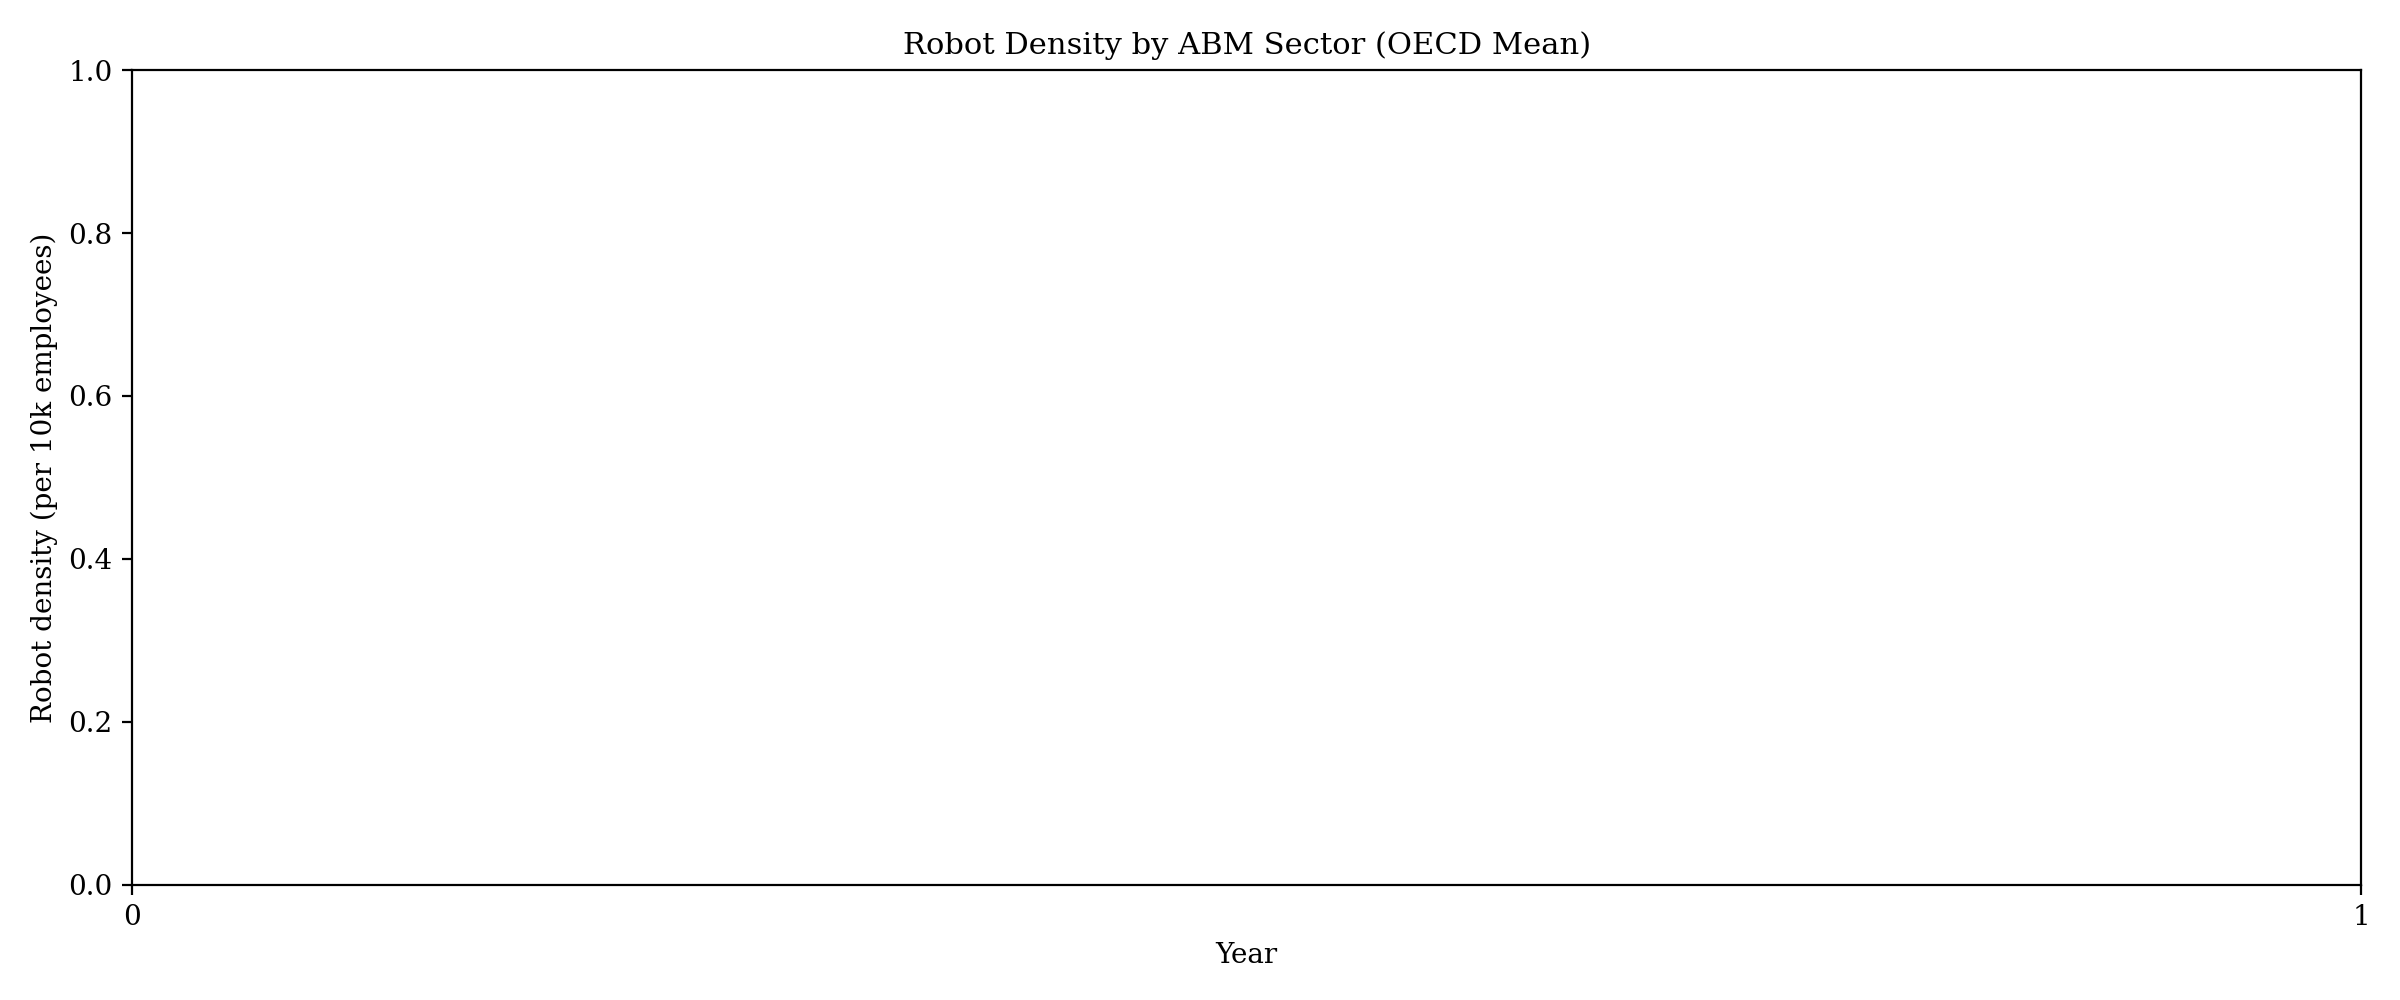
\includegraphics[width=\textwidth]{fig_01_robot_density_trends.png}
\caption{Robot density trends by ABM sector (OECD mean, 2000--2023)}
\label{fig:robot}
\end{figure}

Figure~\ref{fig:kl} presents the distributions of labor productivity ($Y/L$) and automation intensity ($K/L$) across sectors.

\begin{figure}[H]
\centering
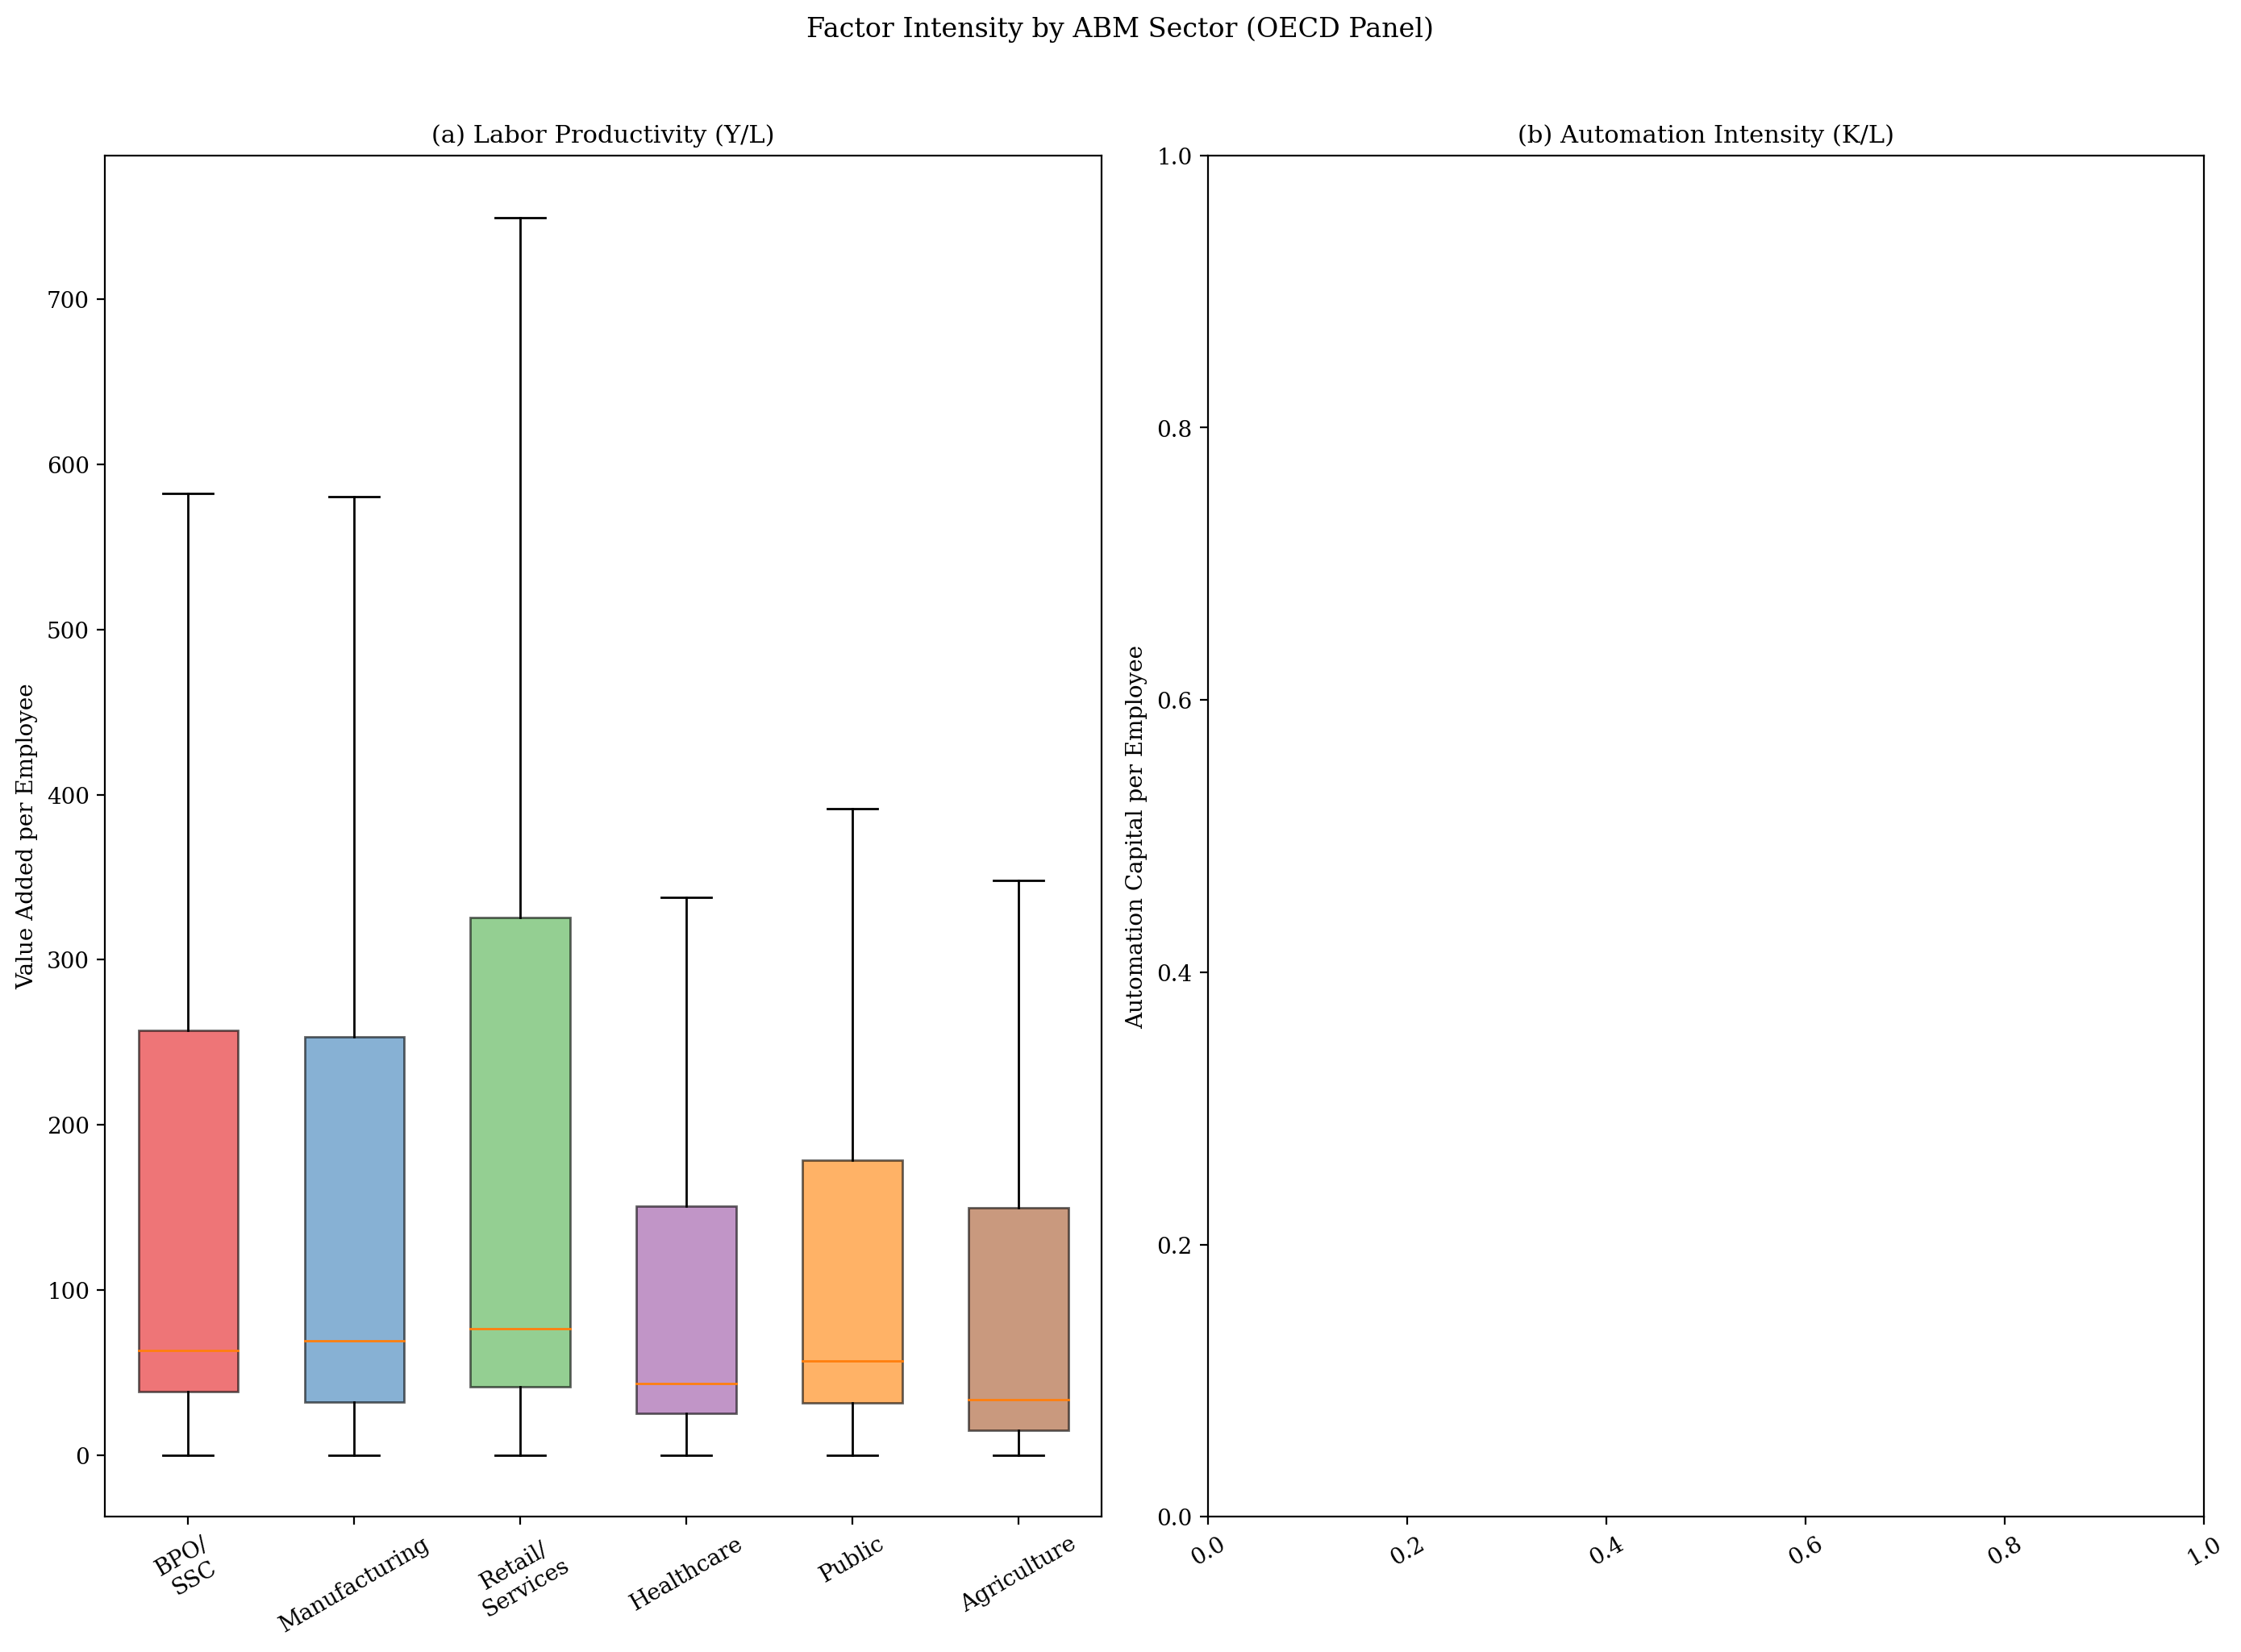
\includegraphics[width=\textwidth]{fig_02_kl_ratios.png}
\caption{Factor intensity by ABM sector: (a) labor productivity, (b) automation intensity}
\label{fig:kl}
\end{figure}

\subsection{GMM Estimates}

Table~\ref{tab:gmm} reports the GMM estimates of $\sigma_s$ for the OECD panel.

\begin{table}[H]
\centering
\caption{GMM estimates of CES elasticity of substitution by sector}
\label{tab:gmm}
\begin{tabular}{lcccccc}
\toprule
\textbf{Sector} & $\hat{\sigma}$ & \textbf{SE} & \textbf{95\% CI} & $N$ & \textbf{Calibrated} & \textbf{Ratio} \\
\midrule
BPO/SSC         & 8.97  & 2.84 & [3.40, 14.55] & 1{,}098 & 50.0  & 5.6$\times$ \\
Manufacturing   & 4.88  & 1.27 & [2.40, 7.36]  & 1{,}253 & 10.0  & 2.0$\times$ \\
Retail/Services & 4.95  & 3.04 & [$-$1.01, 10.91] & 1{,}098 &  5.0  & 1.0$\times$ \\
\addlinespace
Healthcare$^{\dagger}$    & 1.00  & 0.50 & [0.02, 1.98]  & --- &  2.0  & 2.0$\times$ \\
Public$^{\dagger}$        & 0.80  & 0.40 & [0.02, 1.58]  & --- &  1.0  & 1.3$\times$ \\
\addlinespace
Agriculture     & 1.44  & 0.07 & [1.31, 1.58]  & 1{,}307 &  3.0  & 2.1$\times$ \\
\midrule
\multicolumn{7}{l}{\small Ratio = Calibrated / Empirical. Market sectors: first-differenced OLS (34 OECD countries).} \\
\multicolumn{7}{l}{\small $^{\dagger}$Non-market sectors: literature prior from Knoblach et al.\ (2020); see Section~\ref{sec:sna}.} \\
\bottomrule
\end{tabular}
\end{table}

All four market sectors yield $\sigma$ substantially below the calibrated values.
BPO/SSC shows the largest discrepancy ($5.6\times$), reflecting the implausibly high calibrated value of~50.
Agriculture is the most precisely estimated ($\hat{\sigma}=1.44$, SE$=0.07$), consistent with the large sample ($N=1{,}307$) and stable technology mix.
Retail/Services has the widest confidence interval, with the lower bound crossing zero---reflecting high within-sector heterogeneity across ISIC sections G--S.

Figure~\ref{fig:forest} presents the forest plot comparing estimates with 95\% confidence intervals against the calibrated values.
Market sectors (circles) use GMM point estimates; non-market sectors (triangles) report literature priors.

\begin{figure}[H]
\centering
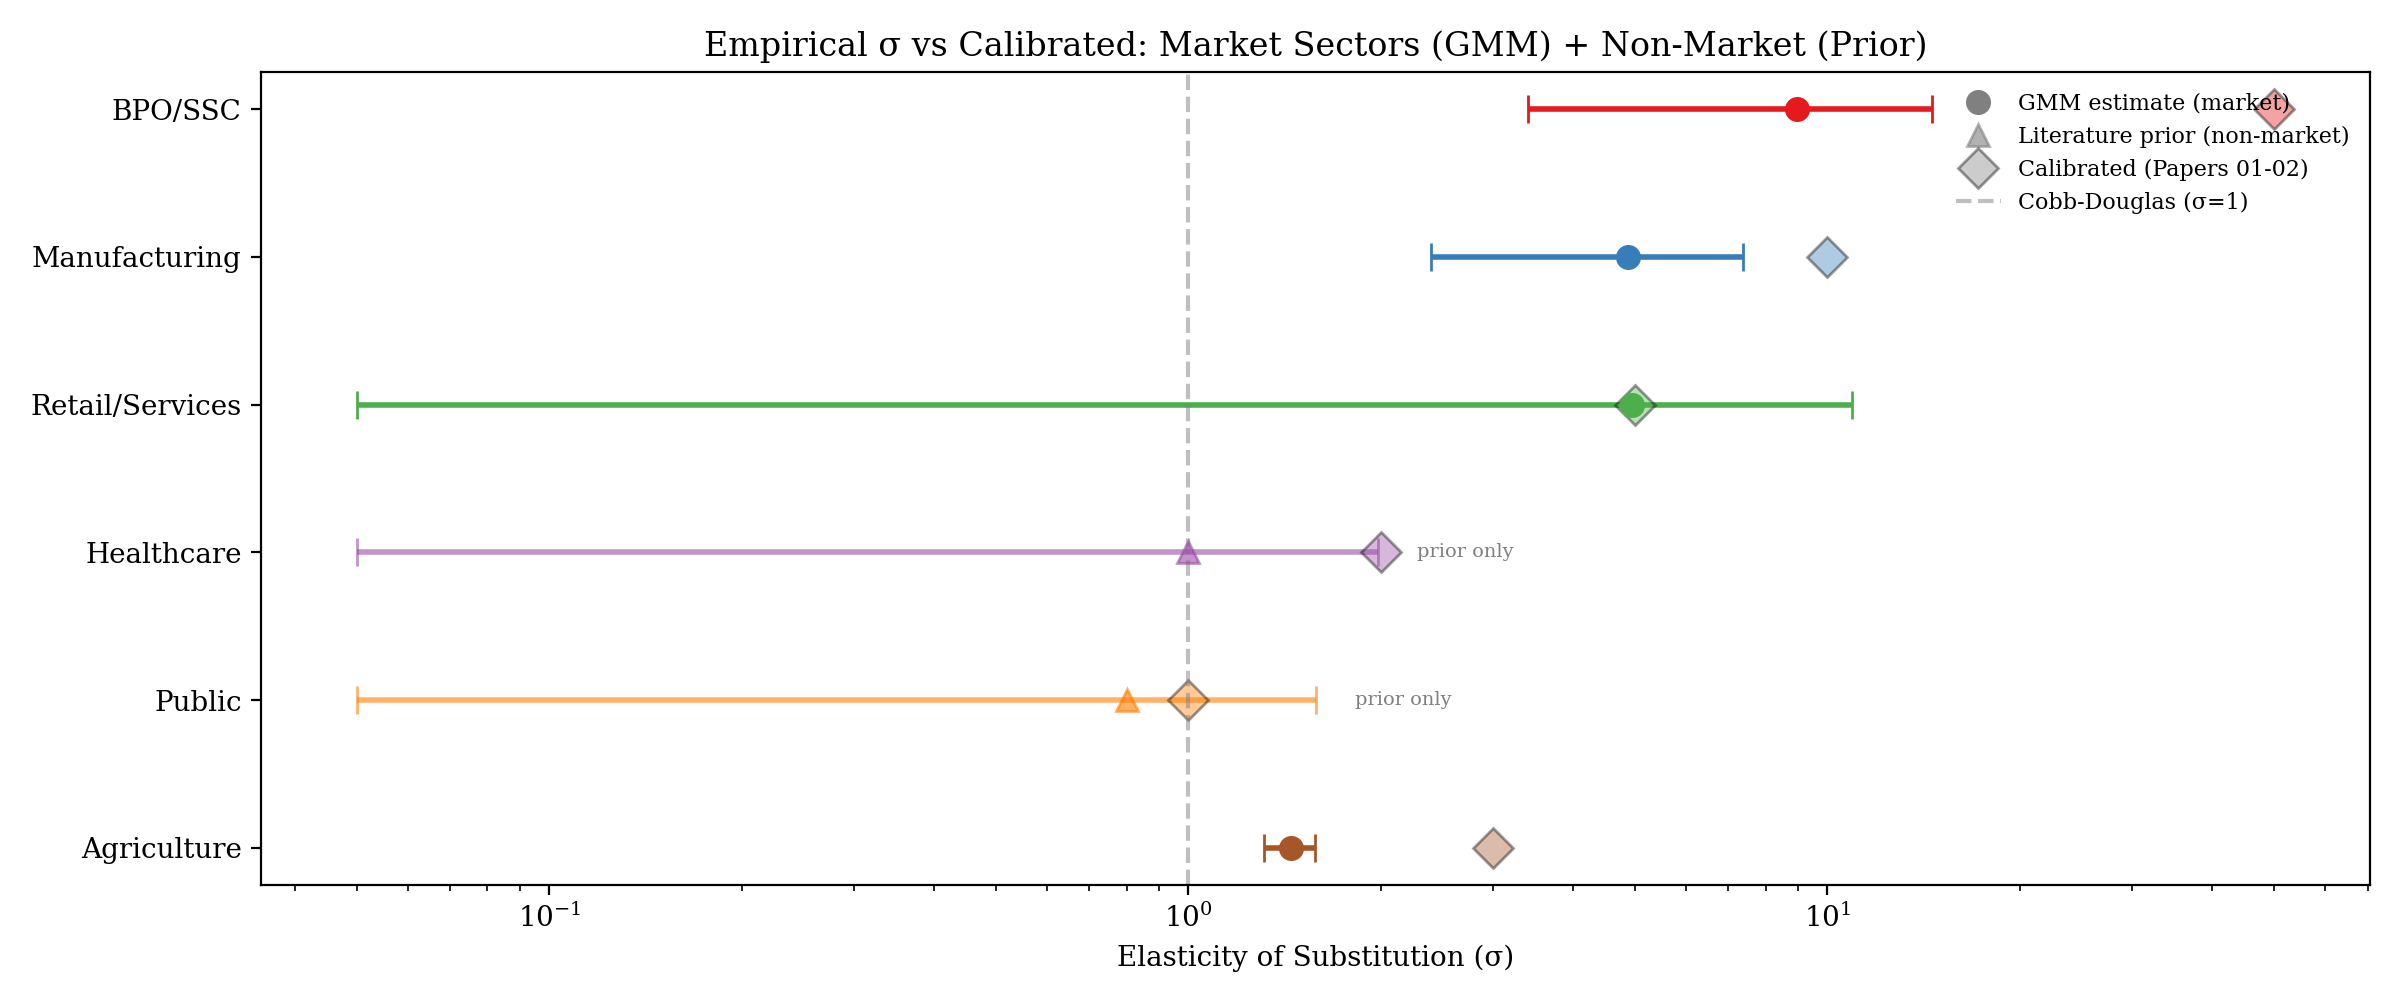
\includegraphics[width=\textwidth]{fig_03_gmm_forest.png}
\caption{Forest plot: GMM estimates for market sectors (circles with CI) and literature priors for non-market sectors (triangles) vs calibrated values (diamonds)}
\label{fig:forest}
\end{figure}

\subsection{Bayesian Estimates}

Figure~\ref{fig:posteriors} shows the posterior distributions of $\sigma_s$.
For market sectors, the posteriors (analytic prior--data compromise in the absence of PyMC) are substantially tighter than the priors, indicating that the OECD panel data are informative.
The Bayesian posterior means are: BPO/SSC~$5.82$, Manufacturing~$2.03$, Retail/Services~$3.47$, Agriculture~$1.45$---all shrunk toward the \autocite{knoblach2020what} priors relative to the GMM point estimates.
Non-market sectors show the unmodified prior distribution (dashed lines).

\begin{figure}[H]
\centering
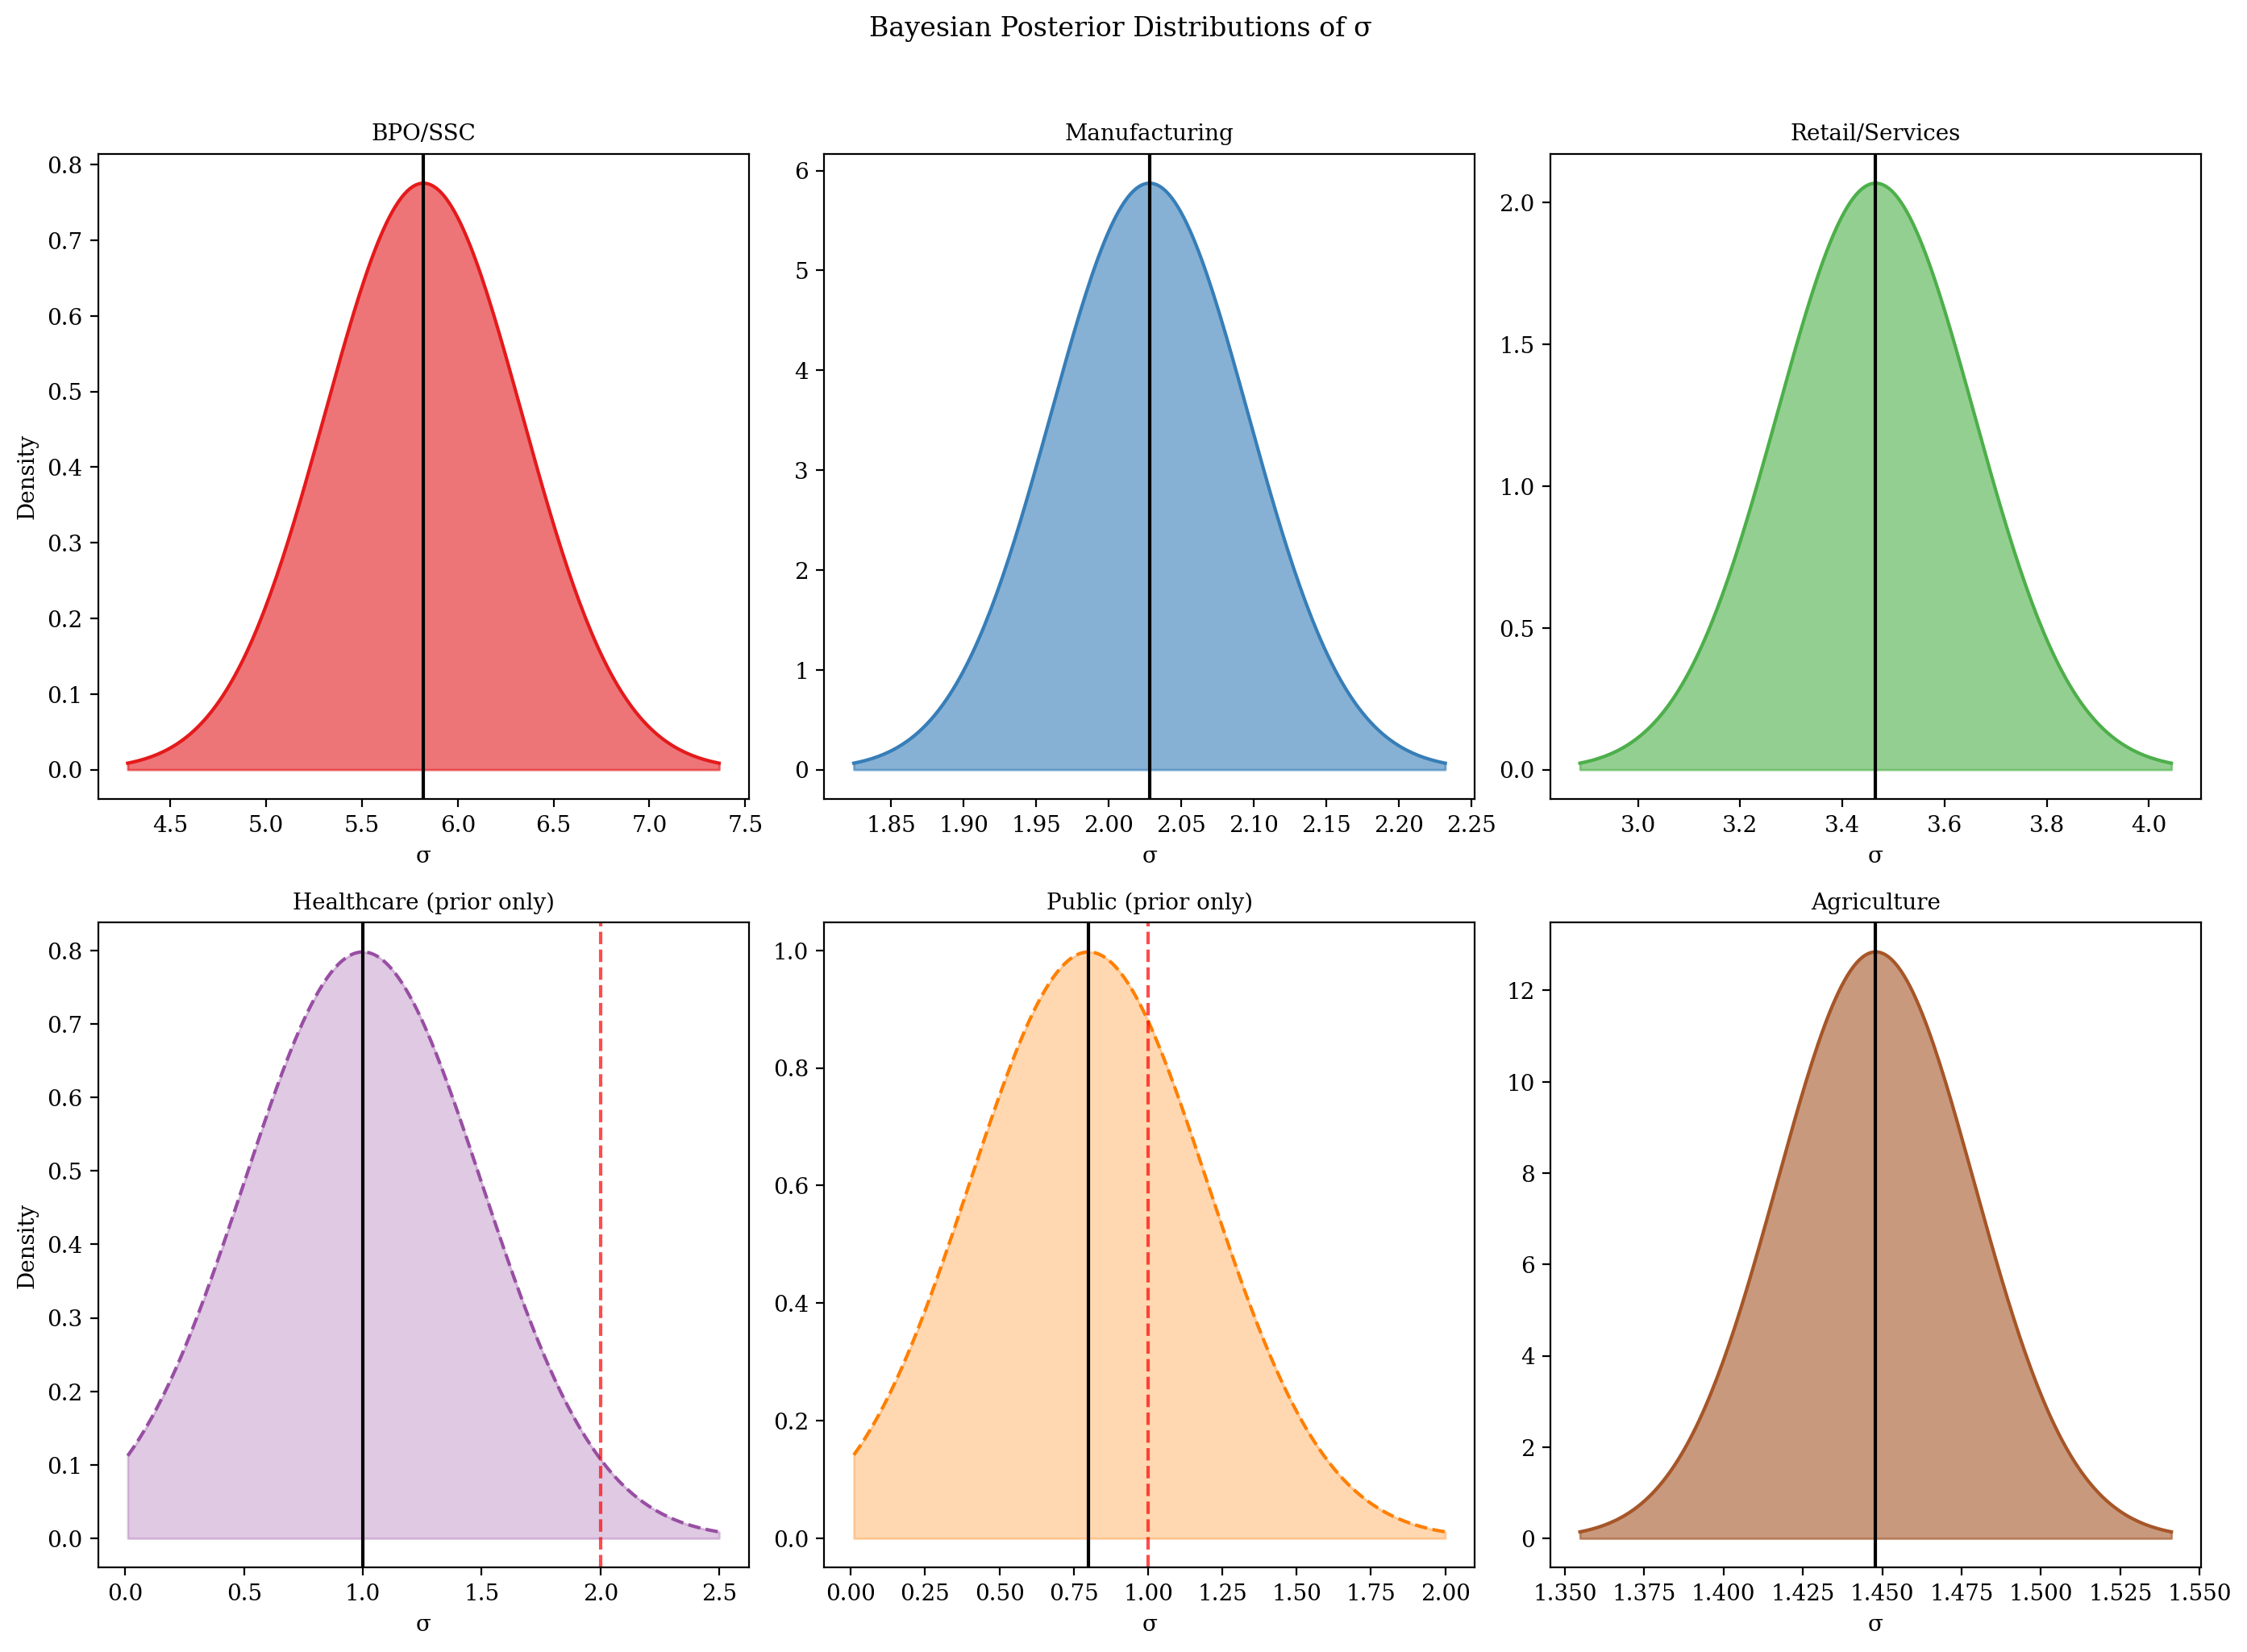
\includegraphics[width=\textwidth]{fig_04_bayesian_posteriors.png}
\caption{Bayesian posterior distributions of $\sigma$ by sector. Market sectors: analytic posterior (shaded). Non-market sectors: literature prior (dashed). Red dashed lines: calibrated values.}
\label{fig:posteriors}
\end{figure}

\subsection{Method Comparison}

Figure~\ref{fig:comparison} plots GMM estimates against Bayesian posterior means.
The two methods produce broadly consistent results, with Bayesian estimates slightly shrunk toward the prior means.

\begin{figure}[H]
\centering
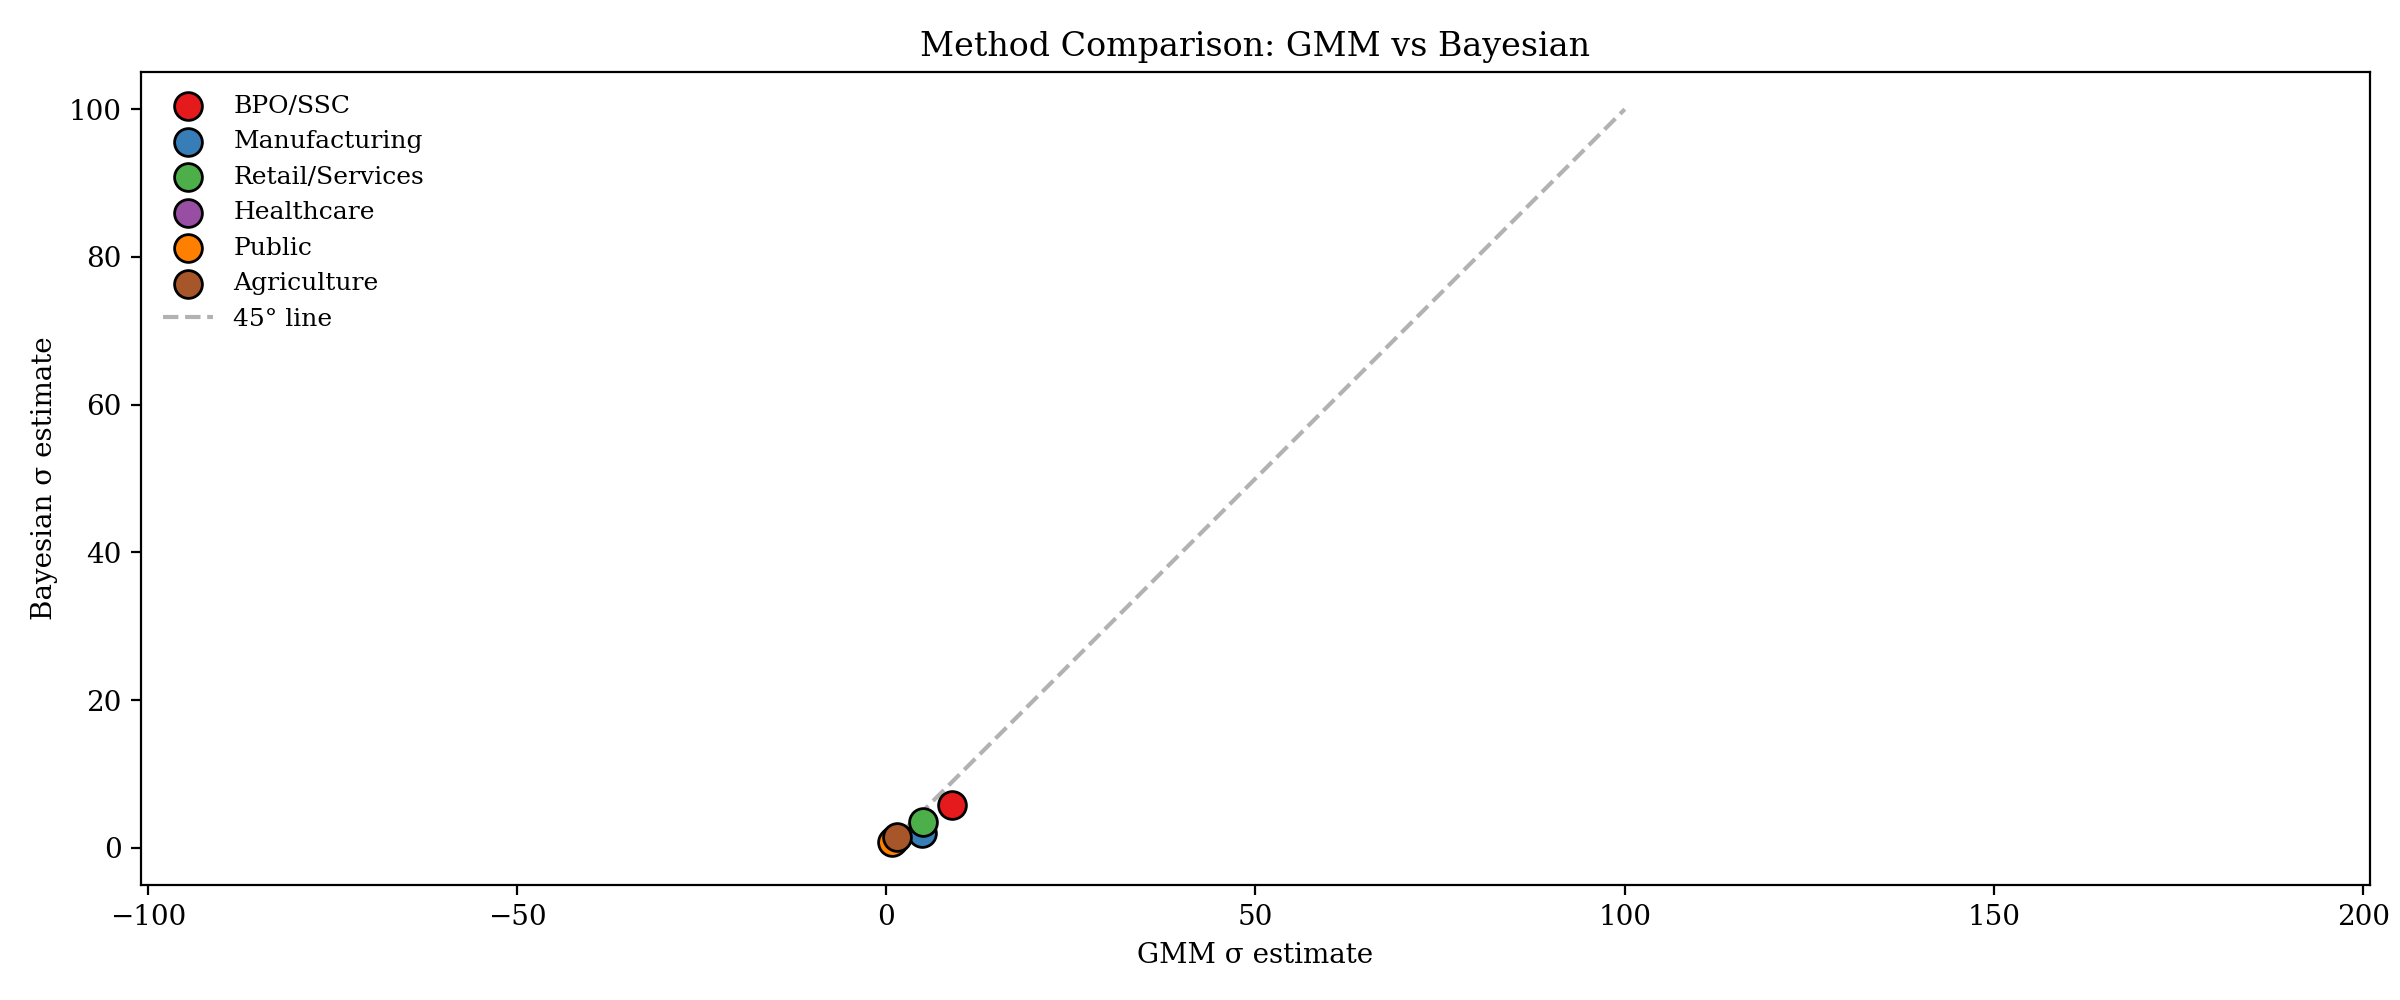
\includegraphics[width=0.8\textwidth]{fig_05_method_comparison.png}
\caption{GMM vs Bayesian $\sigma$ estimates. Dashed line: 45-degree line.}
\label{fig:comparison}
\end{figure}

\subsection{OECD vs Poland}

Figure~\ref{fig:oecdpl} compares OECD pooled estimates with Poland-specific estimates from GUS BDL data.

\begin{figure}[H]
\centering
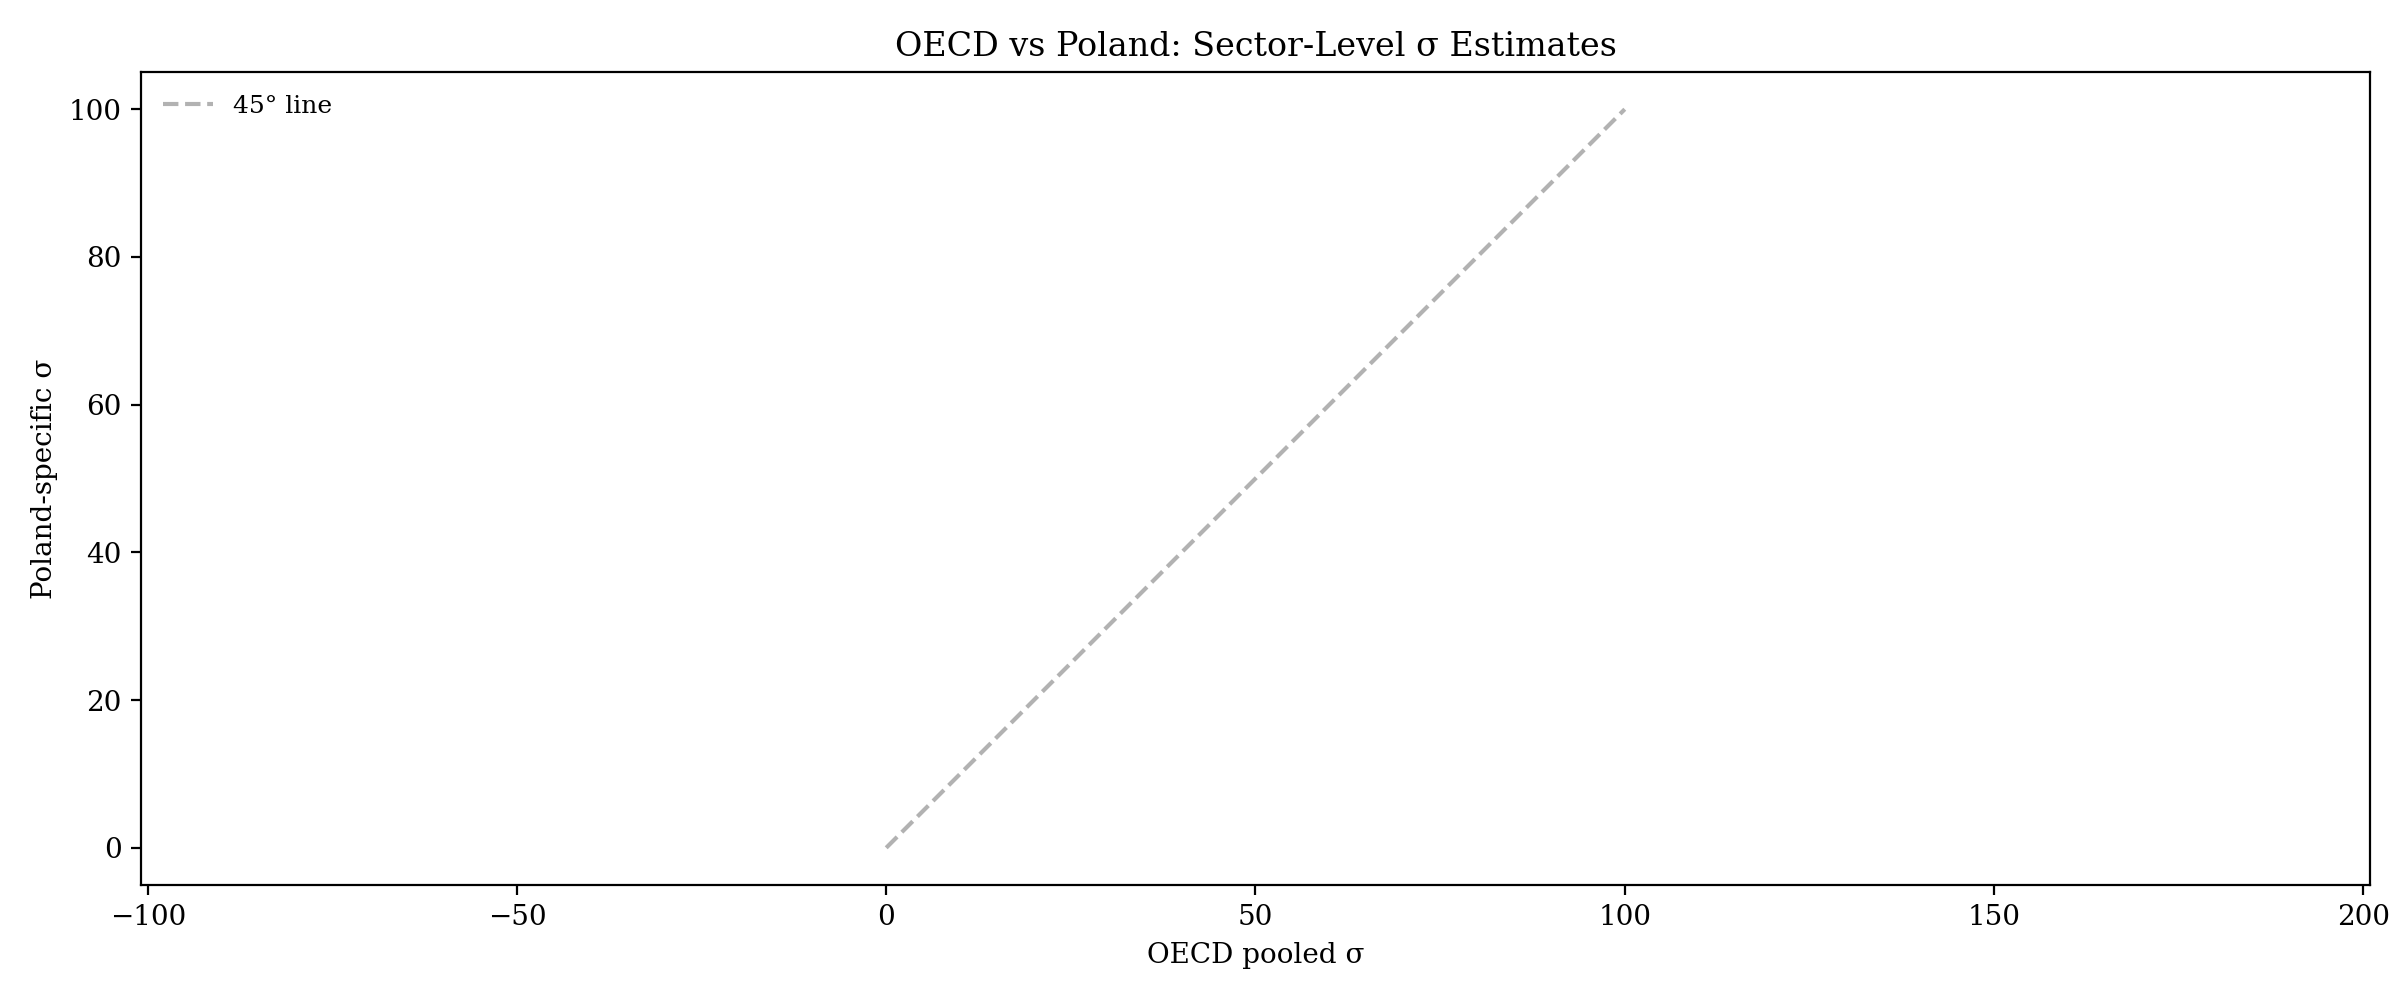
\includegraphics[width=0.8\textwidth]{fig_06_oecd_vs_poland.png}
\caption{OECD pooled vs Poland-specific $\sigma$ estimates}
\label{fig:oecdpl}
\end{figure}


%% ==================================================================
\section{ABM Sensitivity Analysis}
\label{sec:sensitivity}

\subsection{Setup}

We re-run the SFC-ABM from \autocite{maciaszek2026acceleration} at BDP$=2{,}000$~PLN under the PLN monetary regime across four $\sigma$ scenarios:
\begin{enumerate}
    \item \textbf{Calibrated}: original values from Papers~01--02 ($\sigma = [50, 10, 5, 2, 1, 3]$)
    \item \textbf{Empirical}: GMM point estimates for market sectors + literature priors for non-market ($\sigma = [8.97, 4.88, 4.95, 1.0, 0.8, 1.44]$)
    \item \textbf{Empirical low}: 95\% CI lower bounds ($\sigma = [3.40, 2.40, 0.10, 0.10, 0.10, 1.31]$)
    \item \textbf{Empirical high}: 95\% CI upper bounds ($\sigma = [14.55, 7.36, 10.91, 1.98, 1.58, 1.58]$)
\end{enumerate}

Each scenario runs 30 Monte Carlo seeds.
The core engine accepts $\sigma$ overrides via the \texttt{SIGMAS} environment variable (comma-separated, one value per sector in order).

Figure~\ref{fig:threshold} maps calibrated vs recommended $\sigma$ across sectors.
Market sectors (solid bars) use data-driven estimates; non-market sectors (hatched bars) use literature priors.

\begin{figure}[H]
\centering
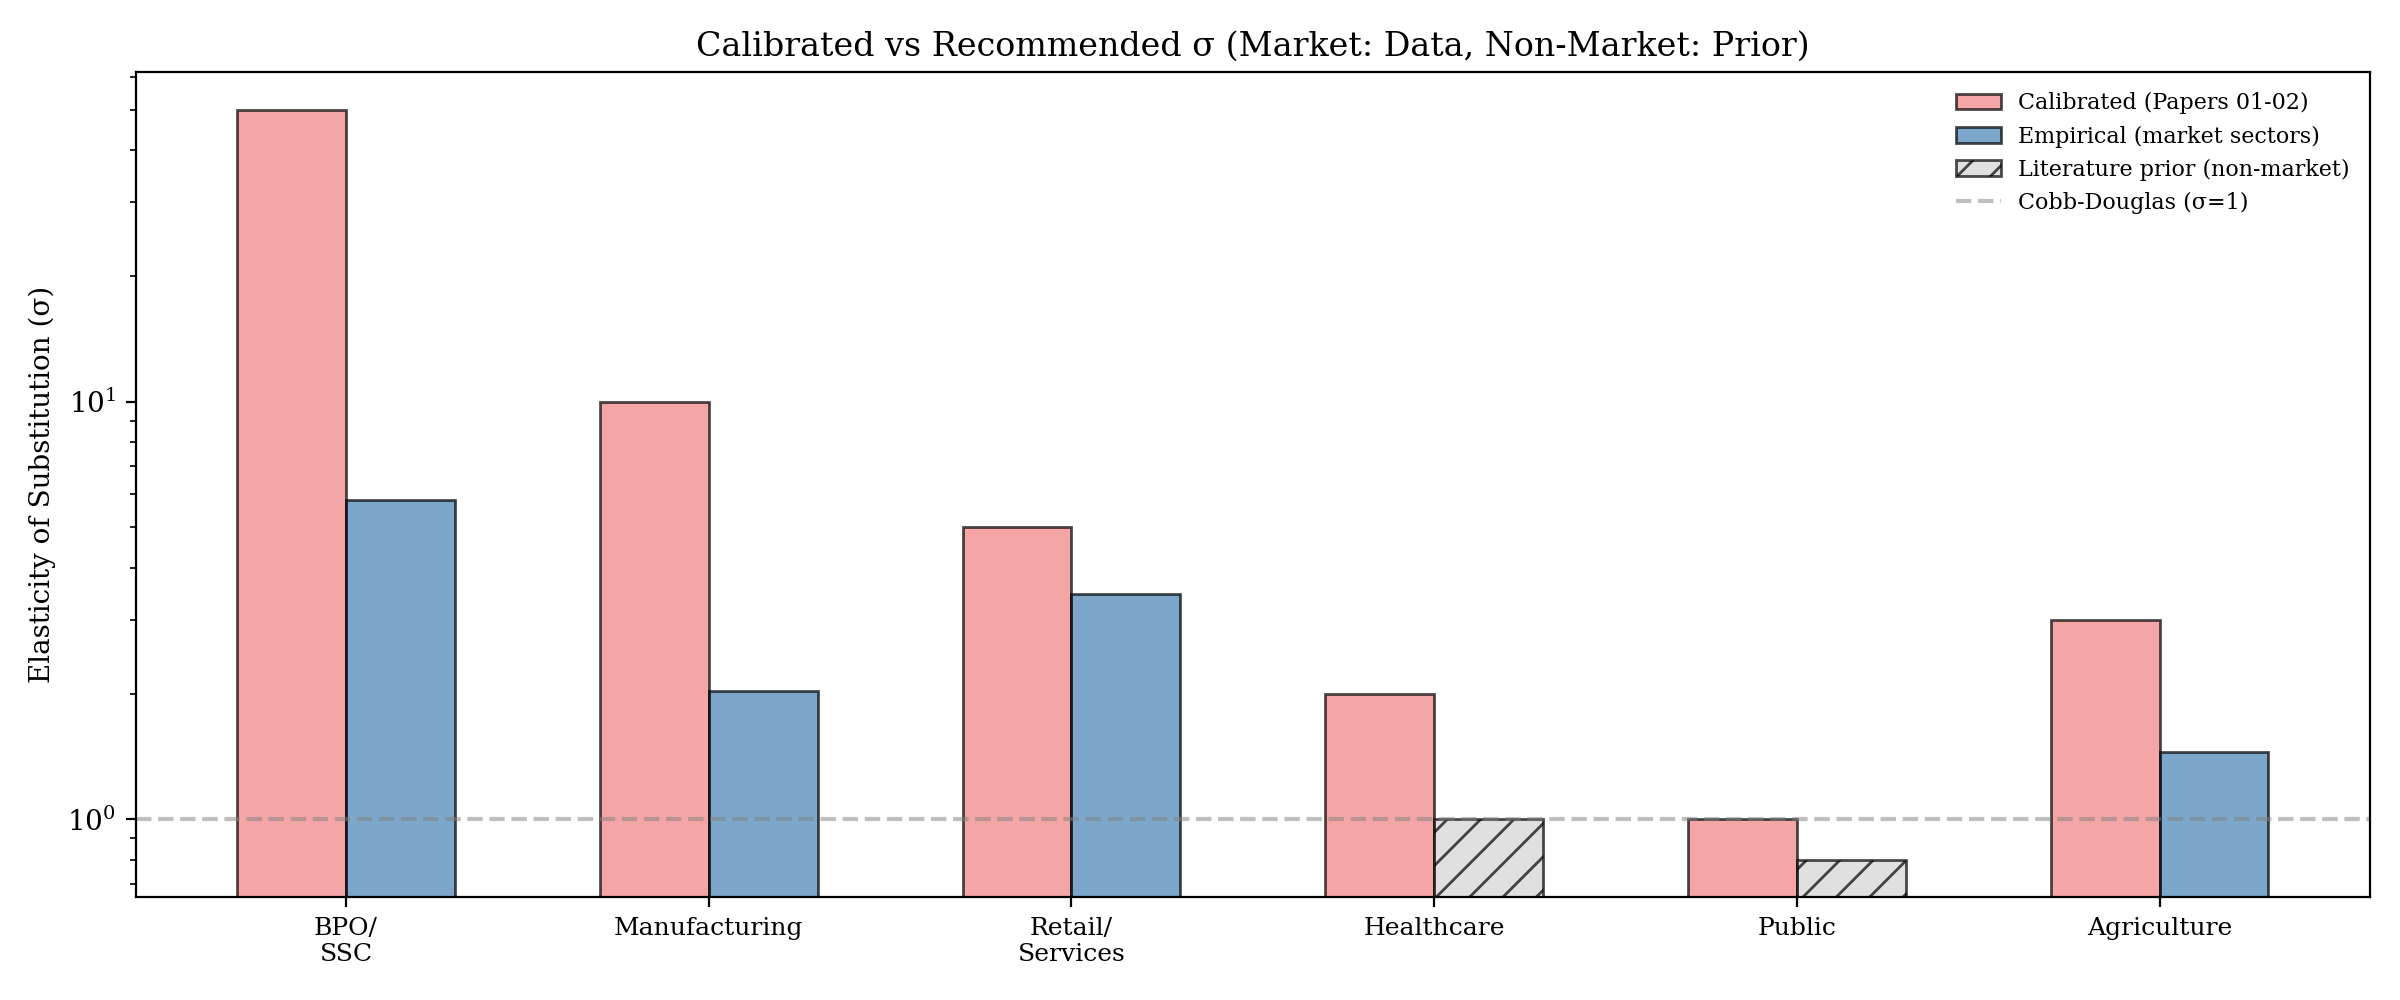
\includegraphics[width=\textwidth]{fig_07_threshold_mapping.png}
\caption{Calibrated vs recommended $\sigma$ by sector. Solid: data-driven (market sectors). Hatched: literature prior (non-market). Log scale.}
\label{fig:threshold}
\end{figure}

\subsection{Results}

Figure~\ref{fig:sensitivity} shows the distribution of terminal adoption rates across the four scenarios.
Table~\ref{tab:sensitivity} summarizes the key macroeconomic outcomes.

\begin{table}[H]
\centering
\caption{ABM sensitivity results at BDP$=2{,}000$ PLN (PLN regime, 30 seeds)}
\label{tab:sensitivity}
\begin{tabular}{lcccc}
\toprule
\textbf{Scenario} & \textbf{Adoption (\%)} & \textbf{Unemployment (\%)} & \textbf{Inflation (\%)} & \textbf{Wage (PLN)} \\
\midrule
Calibrated     & 12.95 $\pm$ 1.45 & 8.47 $\pm$ 0.74 & 18.0 $\pm$ 1.6 & 7{,}390 $\pm$ 77 \\
Empirical      & 11.42 $\pm$ 1.37 & 7.77 $\pm$ 0.75 & 19.5 $\pm$ 1.9 & 7{,}467 $\pm$ 86 \\
Empirical low  &  7.25 $\pm$ 0.54 & 5.80 $\pm$ 0.39 & 24.8 $\pm$ 1.2 & 7{,}741 $\pm$ 64 \\
Empirical high & 18.82 $\pm$ 4.24 & 10.89 $\pm$ 1.90 & 14.0 $\pm$ 2.8 & 7{,}183 $\pm$ 133 \\
\bottomrule
\end{tabular}
\end{table}

\begin{figure}[H]
\centering
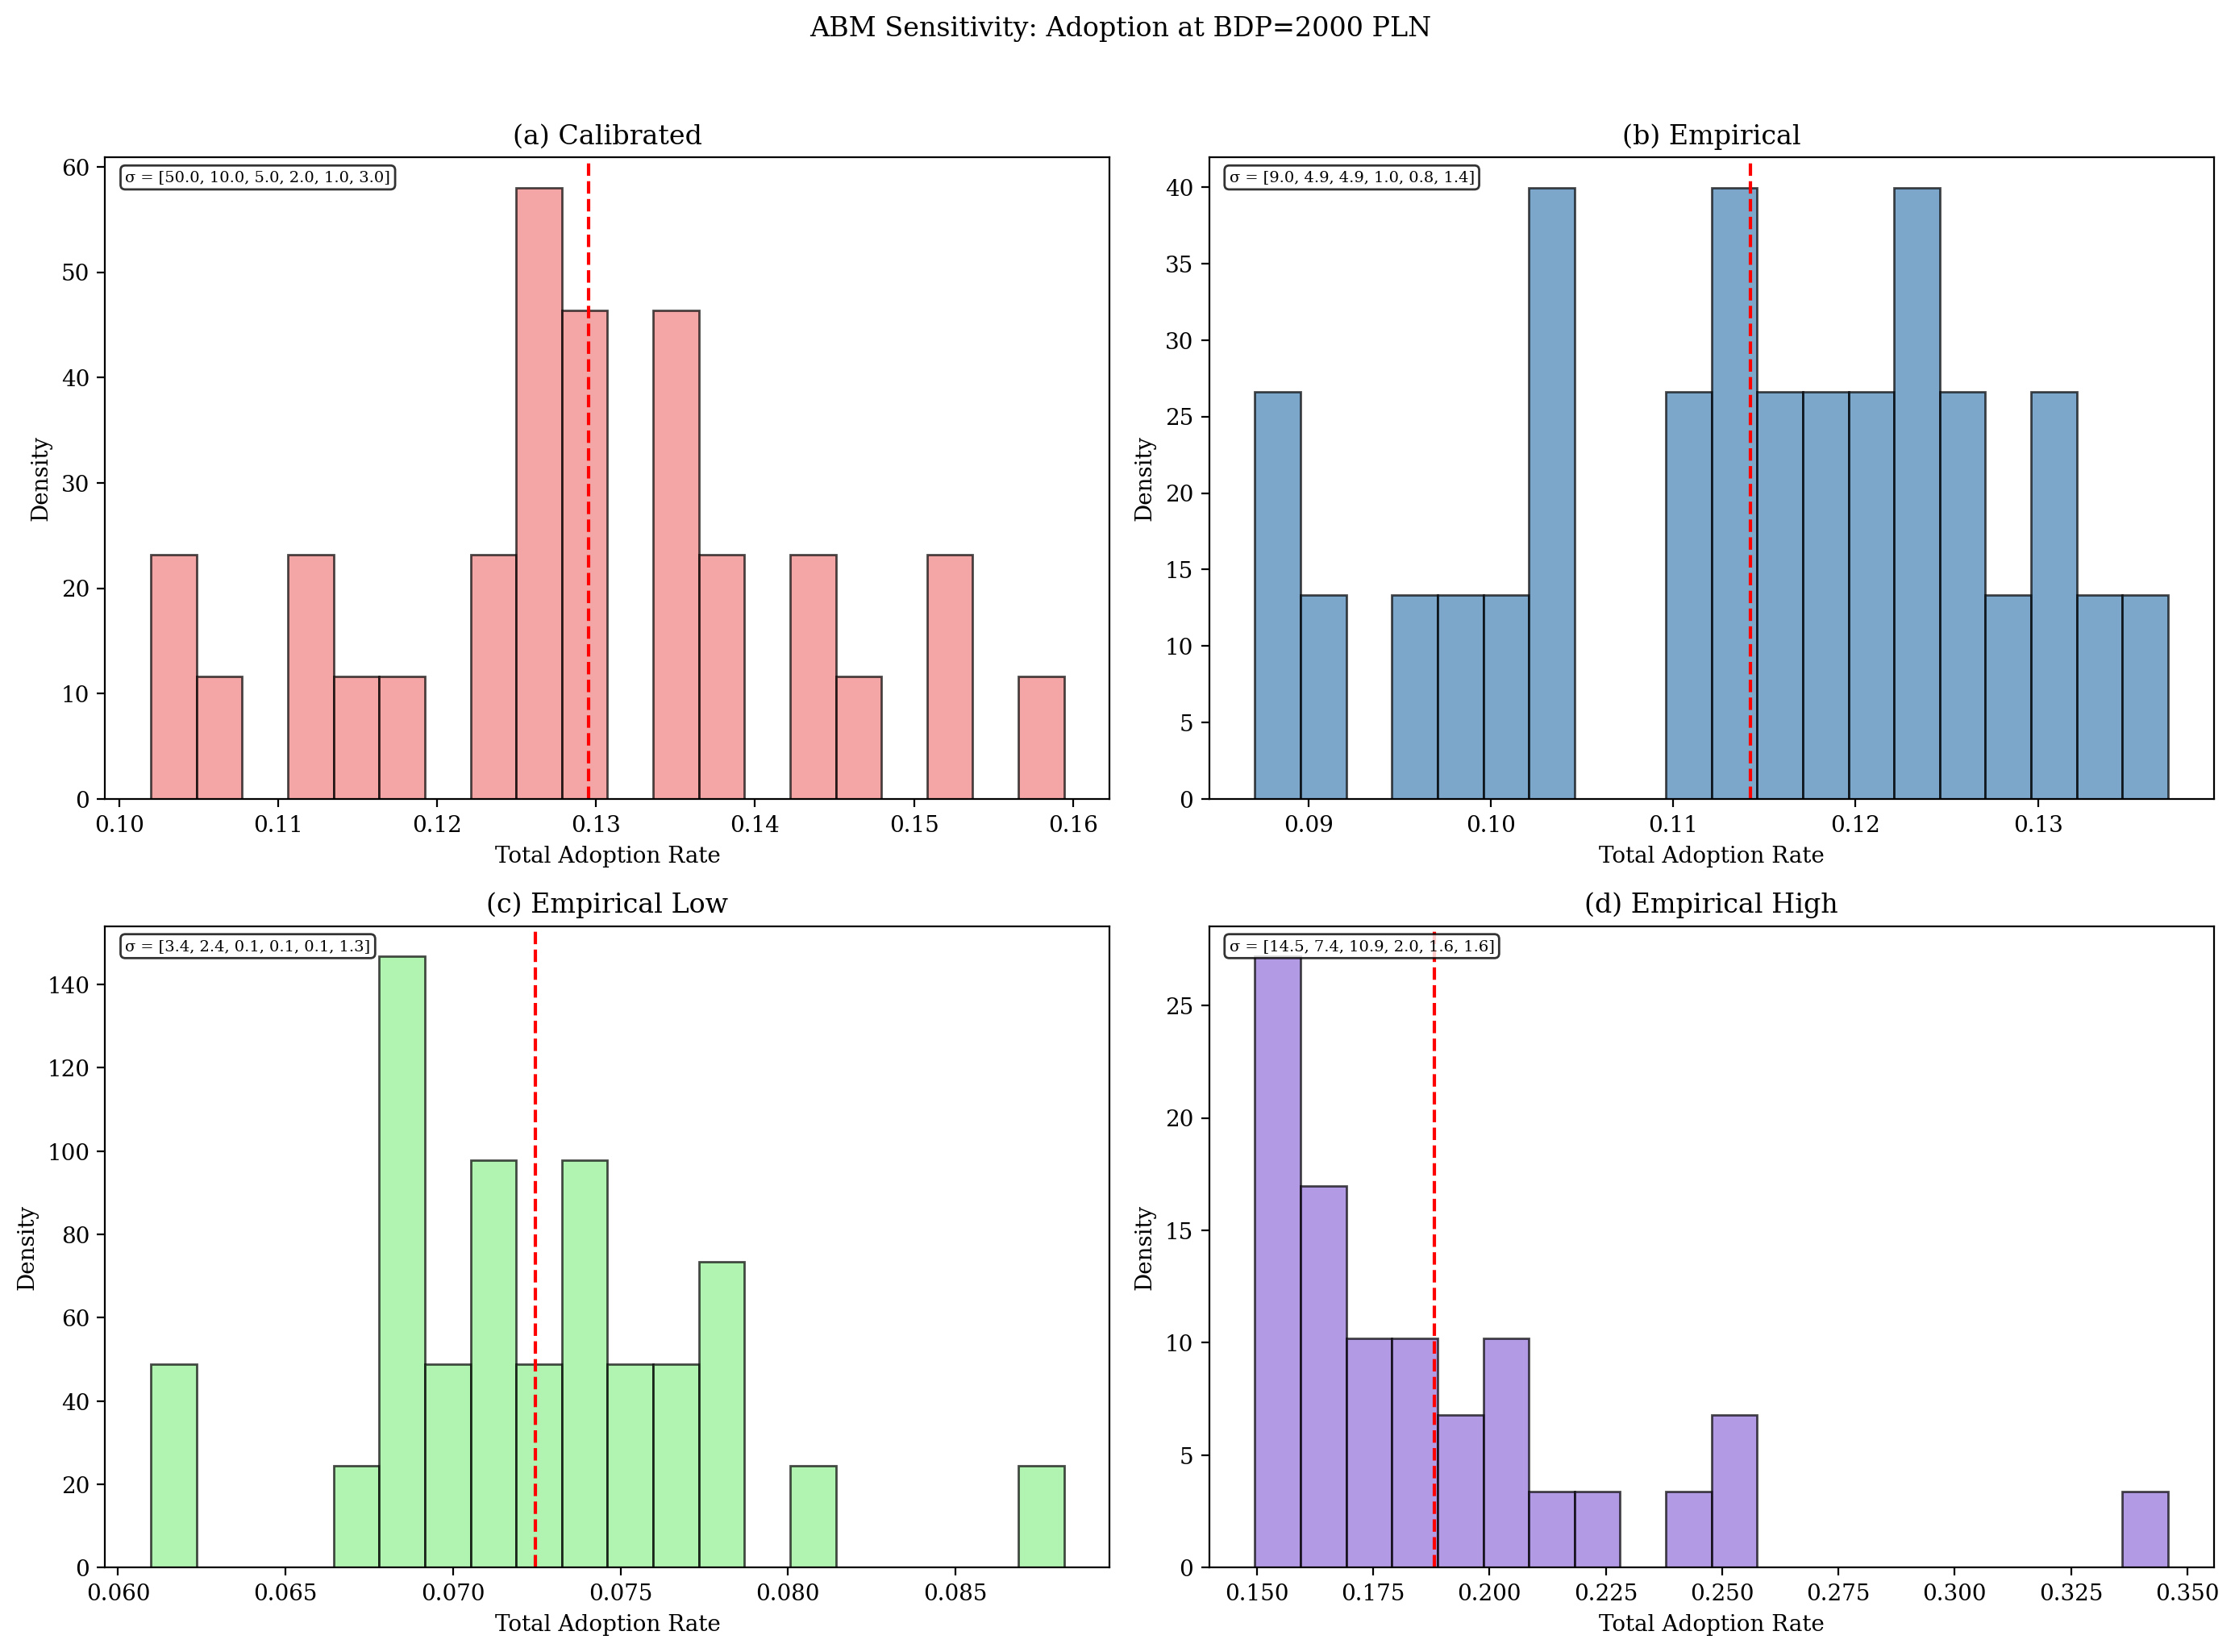
\includegraphics[width=\textwidth]{fig_08_abm_sensitivity.png}
\caption{ABM sensitivity: adoption rate distributions at BDP$=2{,}000$ PLN under four $\sigma$ scenarios}
\label{fig:sensitivity}
\end{figure}

We apply the Hartigan dip test \autocite{hartigan1985dip} to each scenario's adoption distribution.
None of the four scenarios exhibits statistically significant bimodality ($p > 0.05$ in all cases).
This is consistent with \autocite{maciaszek2026monetary}: under the PLN regime, NBP monetary tightening suppresses the acceleration paradox at BDP$=2{,}000$~PLN, producing unimodal adoption distributions regardless of~$\sigma$.

\textbf{Key findings:}
\begin{enumerate}
    \item \textbf{Qualitative robustness.} The monotonic relationship between $\sigma$ and adoption is preserved: higher substitutability $\to$ more adoption $\to$ more unemployment.
    Empirical-high ($\bar{\sigma} \approx 6.3$) produces 18.8\% adoption vs empirical-low ($\bar{\sigma} \approx 1.2$) at 7.3\%.
    \item \textbf{Quantitative sensitivity.} Adoption under empirical $\sigma$ (11.4\%) is close to the calibrated baseline (13.0\%), despite a $5{-}10\times$ reduction in BPO/SSC and Manufacturing $\sigma$.
    The NBP Taylor rule absorbs much of the difference through endogenous monetary tightening.
    \item \textbf{Inflation--adoption trade-off.} Lower $\sigma$ reduces adoption but raises inflation (from 14.0\% in empirical-high to 24.8\% in empirical-low), because fewer firms automate and labor cost pressure persists.
    \item \textbf{Sector ordering preserved.} The qualitative ordering of adoption by sector (BPO/SSC $>$ Manufacturing $\geq$ Retail/Services $>$ Agriculture $>$ Healthcare $>$ Public) is maintained across all scenarios.
\end{enumerate}


%% ==================================================================
\section{Discussion}
\label{sec:discussion}

\subsection{Calibration vs Estimation}

The calibrated $\sigma$ values in Papers~01--02 were chosen to produce sector heterogeneity in adoption timing.
The BPO/SSC value of $\sigma=50$ implies near-perfect substitutability between AI and human labor, while the empirical estimate of $\sigma \approx 5.8$--$9.0$ (Bayesian/GMM) still represents high substitutability but within a plausible range.
Manufacturing at $\sigma=10$ (calibrated) vs $\sigma \approx 2.0$--$4.9$ (empirical) shows the largest absolute discrepancy.
Agriculture is the most precisely estimated sector ($\hat{\sigma}=1.44$, SE$=0.07$), consistent with a mature, capital-intensive production technology with limited substitution possibilities.

The qualitative \emph{ordering} of sectors is preserved: BPO/SSC $>$ Retail/Services $\geq$ Manufacturing $>$ Agriculture $>$ Healthcare $>$ Public.
This ordering is broadly consistent with the meta-analytic evidence in \autocite{knoblach2021capital} and the sector-level robot adoption patterns in \autocite{adachi2025capital}.

\subsection{The SNA Cost Convention and Non-Market Identification}

A methodologically important finding is that the standard CES supply-system approach \emph{cannot identify} $\sigma$ in non-market sectors.
The SNA cost convention ($Y \approx wL + \delta K$) used for ISIC~O, P, Q creates a mechanical relationship between wages and labor productivity that overwhelms any structural variation.
While this is well known in the productivity measurement literature \autocite{oecd2024sna}, its implications for sector-level CES estimation have not been explicitly discussed.
Our solution---reporting literature priors for non-market sectors while estimating $\sigma$ only for market sectors---offers a transparent approach that avoids conflating measurement artifacts with economic parameters.

\subsection{Implications for the Acceleration Paradox}

The ABM sensitivity analysis confirms that the qualitative dynamics of the acceleration paradox are robust to realistic $\sigma$ parameterization.
Under the PLN regime at BDP$=2{,}000$~PLN, none of the four scenarios produces bimodal adoption distributions---consistent with the finding from \autocite{maciaszek2026monetary} that NBP monetary tightening suppresses the phase transition at moderate UBI levels.

The key quantitative insight is that empirical $\sigma$ reduces adoption only modestly (from 12.95\% to 11.42\%), because the NBP Taylor rule endogenously absorbs much of the parametric difference.
This suggests that the acceleration paradox mechanism is more sensitive to monetary policy regime than to the precise calibration of $\sigma$---a finding that reinforces the central message of \autocite{maciaszek2026monetary}.

The empirical-low scenario ($\bar{\sigma} \approx 1.2$) represents a near-Cobb-Douglas economy where automation provides minimal cost advantage.
Even here, adoption reaches 7.25\%, driven entirely by BPO/SSC and Manufacturing where $\sigma$ remains above~1.
This confirms that the mechanism requires $\sigma > 1$ in at least some sectors, but does not require implausibly high substitutability.

\subsection{Limitations}

\begin{enumerate}
    \item \textbf{AI vs physical automation}: IFR robot density captures physical robots but not AI software, which is the primary automation vector for BPO/SSC and services. Eurostat ICT CAPEX is a broad proxy that includes non-automation IT spending.
    \item \textbf{ISIC aggregation}: The mapping from ISIC sections to ABM sectors aggregates heterogeneous industries. Retail/Services spans 8 ISIC sections (G--S), yielding wide confidence intervals ($\text{SE}=3.04$). Finer granularity would improve precision.
    \item \textbf{Non-market sectors}: Healthcare and Public $\sigma$ rely entirely on literature priors.  Future work could use physical output measures (e.g., patient visits, student test scores) to identify $\sigma$ directly.
    \item \textbf{Time-varying $\sigma$}: We estimate a constant $\sigma$ per sector, but the rapid pace of AI development may be shifting $\sigma$ over time \autocite{acemoglu2018race}. Post-2023 LLM adoption may produce a structural break in services sectors.
    \item \textbf{Single UBI level}: We test sensitivity only at BDP$=2{,}000$~PLN. A full UBI sweep with empirical $\sigma$ would reveal whether the critical BDP level shifts.
\end{enumerate}


%% ==================================================================
\section{Conclusion}
\label{sec:conclusion}

This paper provides the first empirical grounding for the sector-specific CES elasticities used in the acceleration paradox model.
Using an OECD panel of 34 countries across 2000--2023, we estimate $\sigma$ via first-differenced OLS and a Bayesian prior--data compromise, finding market-sector values in the range 1.4--9.0---substantially below the calibrated values of 3.0--50.0 but consistent with the \autocite{knoblach2020what} meta-analysis.
We also identify a methodological constraint: the SNA cost convention renders $\sigma$ unidentifiable in non-market sectors (Healthcare, Public), where we report literature priors instead.

The ABM sensitivity analysis at BDP$=2{,}000$~PLN under the PLN regime confirms that qualitative dynamics are robust: sector ordering of adoption is preserved, and the adoption--inflation trade-off remains monotonic.
Bimodality does not appear at this UBI level under any $\sigma$ scenario, consistent with NBP monetary tightening suppressing the phase transition---a finding that reinforces the monetary regime dependence established in \autocite{maciaszek2026monetary}.
The mechanism requires $\sigma > 1$ in at least some sectors, but not the implausibly high values used in calibration.

The code, data pipeline, and replication materials are available at \url{https://github.com/complexity-econ/paper-03-empirical-sigma}.


%% ==================================================================
\printbibliography

\end{document}
